\documentclass{beamer}

%copied from tmupackage
\usepackage{amsmath}
\usepackage{amsfonts}
\usepackage{graphics}
\usepackage{verbatim}

\setlength\parindent{0pt}
%end of tmupackage

\usepackage{verbatim}


\author{Ethan McDonald \& Thomas Ulmer}
\title{Reedos So Far}

%% \AtBeginSection[]{
%%   \begin{frame}
%%   \vfill
%%   \centering
%%   \begin{beamercolorbox}[sep=8pt,center,shadow=true,rounded=true]{title}
%%     \usebeamerfont{title}\insertsectionhead\par%
%%   \end{beamercolorbox}
%%   \vfill
%%   \end{frame}
%% }

\begin{document}

\begin{frame}
  \maketitle
\end{frame}

\begin{frame}
  \frametitle{Table of Contents}
  \tableofcontents
\end{frame}

\section{What We've Done}

\begin{frame}
  \frametitle{Pre-boot and Linker}
  \begin{columns}
    \begin{column}{0.5\textwidth}
      Linker script:
      \begin{itemize}
      \item Organize reedos ELF binary to QEMU expectations.\\
      \item Bound symbols to access at runtime.\\
      \item Provide alignment where needed.\\
      \end{itemize}
      Linking required to combine Rust code and Assembly.
    \end{column}

    \begin{column}{0.5\textwidth}
      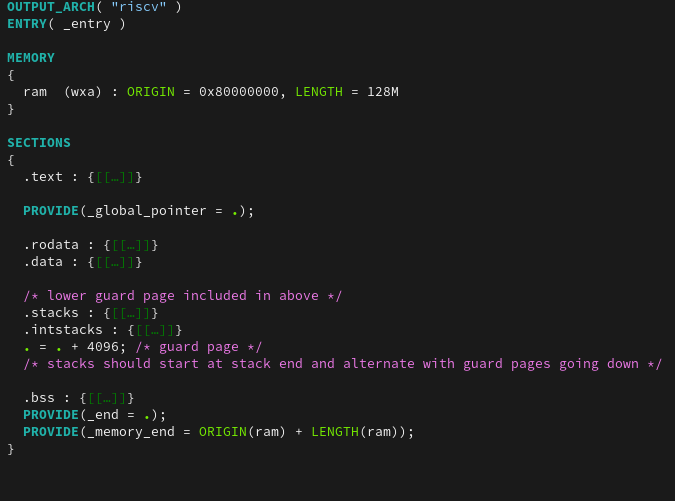
\includegraphics[width=\textwidth]{linker.png}
    \end{column}

  \end{columns}

\end{frame}

\begin{frame}
  \frametitle{Entry into Assembly}
  \begin{columns}
    \begin{column}{0.5\textwidth}
      The first assembly to be run on boot.
      \begin{itemize}
      \item All harts jump to the same place.\\
      \item Set up primary stack and interrupt stack per hart.\\
      \item Prevent harts from colliding in memory.\\
      \item Jump to rust.
      \end{itemize}
    \end{column}
    \begin{column}{0.5\textwidth}
      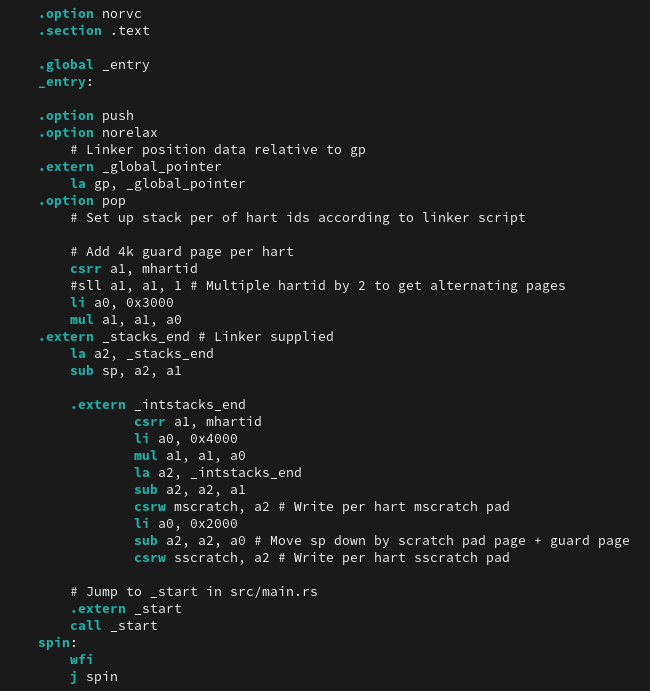
\includegraphics[width=\textwidth]{entry.png}
    \end{column}
  \end{columns}
\end{frame}

\begin{frame}[fragile]
  \frametitle{Start into Rust}
  \begin{columns}
    \begin{column}{0.5\textwidth}
      Setup for transition to supervisor mode
      \begin{itemize}
      \item Disable paging until \begin{verbatim}vm::init\end{verbatim}.\\
      \item Do setup that requires high privilege.\\
      \item ID harts in non-protected register.\\
      \item Begin firing M-mode timer interrupts.
      \end{itemize}
    \end{column}
    \begin{column}{0.5\textwidth}
      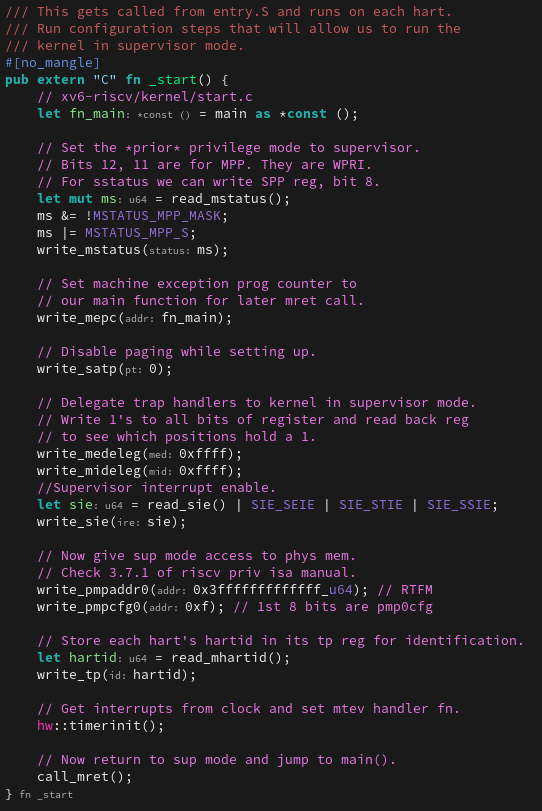
\includegraphics[width=\textwidth]{start.png}
    \end{column}
  \end{columns}
\end{frame}

\begin{frame}
  \frametitle{Main}
  \begin{columns}
    \begin{column}{0.5\textwidth}
      Initialize kernel subsystems on hart 0.
      \begin{itemize}
      \item Devices\\
      \item Exception and Interrupts traps\\
      \item Virtual memory subsystem
      \end{itemize}
    \end{column}
    \begin{column}{0.5\textwidth}
      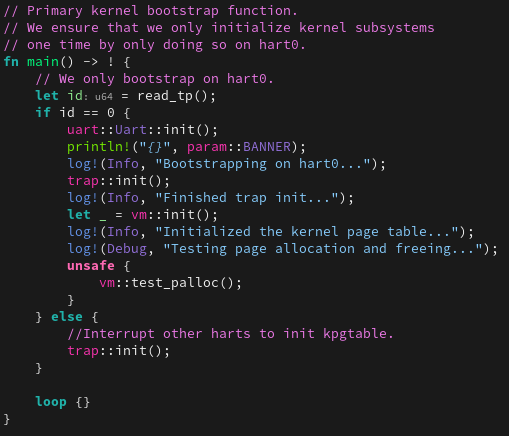
\includegraphics[width=\textwidth]{main.png}
    \end{column}
  \end{columns}
\end{frame}

\begin{frame}[fragile]
  \frametitle{Uart Device}
  \begin{columns}
    \begin{column}{0.5\textwidth}
      Treat serial port as streaming device at byte granularity.
      \begin{itemize}
      \item Initialize to match QEMU\\
      \item Protect with spinlock and hook with \verb_print!_
      \end{itemize}
    \end{column}
    \begin{column}{0.5\textwidth}
      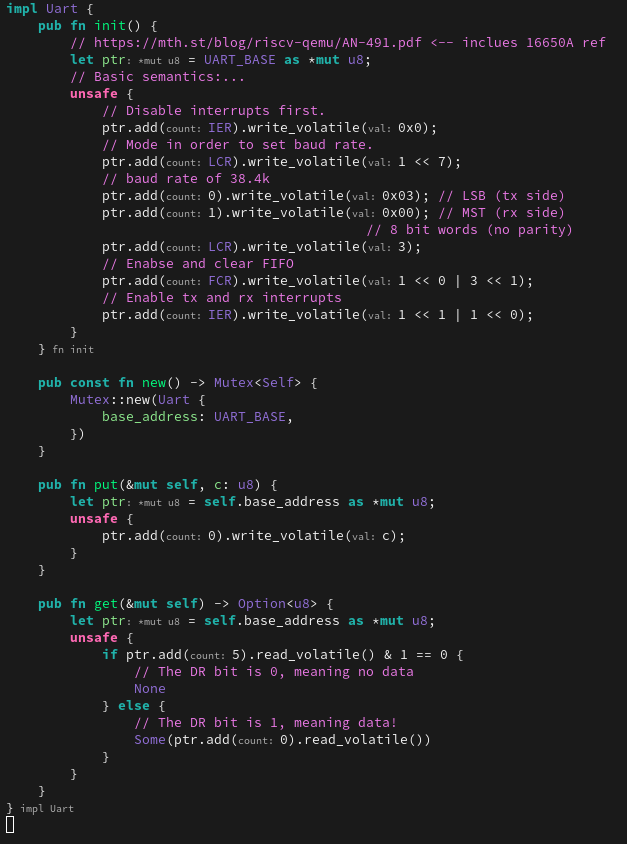
\includegraphics[width=\textwidth]{uart.png}
    \end{column}
  \end{columns}
\end{frame}

\begin{frame}
  \frametitle{Trap into Assembly}
  \begin{columns}
    \begin{column}{0.5\textwidth}
      Middleman between rust and interrupting rust.
      \begin{itemize}
      \item Save registers to allow restoration of previous state.\\
      \item Make it safe to call rust, even if clobbered registers are in use.
      \end{itemize}
    \end{column}
    \begin{column}{0.5\textwidth}
      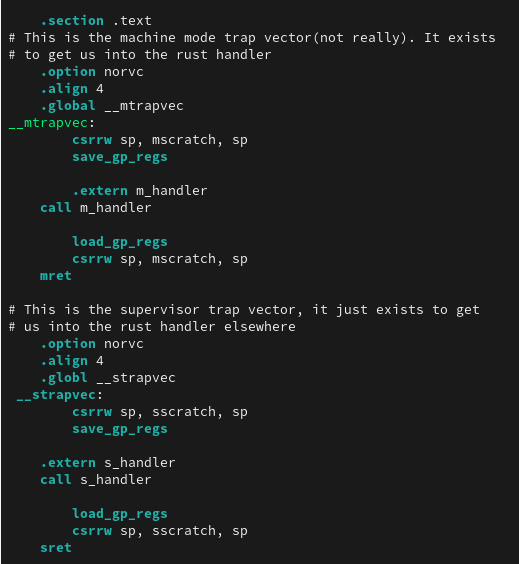
\includegraphics[width=\textwidth]{trapasm.png}
    \end{column}
  \end{columns}
\end{frame}

\begin{frame}[fragile]
  \frametitle{Trap in Rust}
  \begin{columns}
    \begin{column}{0.5\textwidth}
      Switch based on \verb_mcause_ or \verb_scause_
      \begin{itemize}
      \item Reset timer interrupt to make it regularly scheduled.\\
      \item Catch exceptions and halt execution.\\
      \item TODO: catch page faults.
      \end{itemize}
    \end{column}
    \begin{column}{0.5\textwidth}
      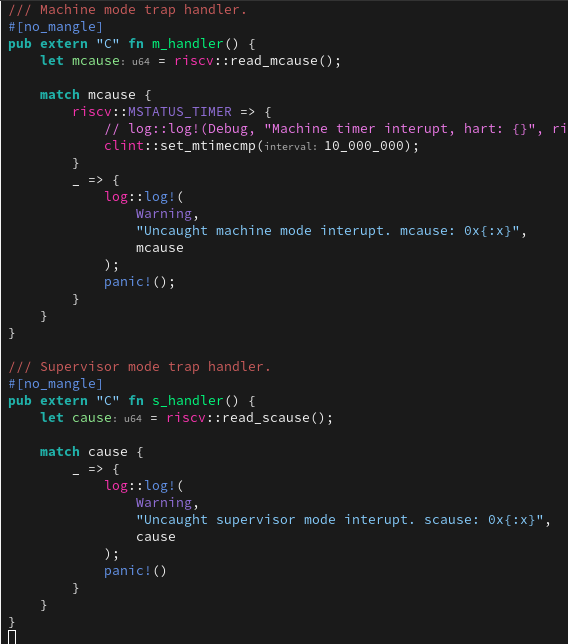
\includegraphics[width=\textwidth]{traprs.png}
    \end{column}
  \end{columns}
\end{frame}

\begin{frame}
  \frametitle{Virtual Memory Subsystem}
  \begin{columns}
    \begin{column}{0.5\textwidth}
      Contains most memory abstractions.
      \begin{itemize}
      \item Page allocation.\\
      \item General allocation.\\
      \item Virtual memory for kernel and processes.\\
      \item Kernel page table maps all of memory with correct permissions.
      \end{itemize}
    \end{column}
    \begin{column}{0.5\textwidth}
      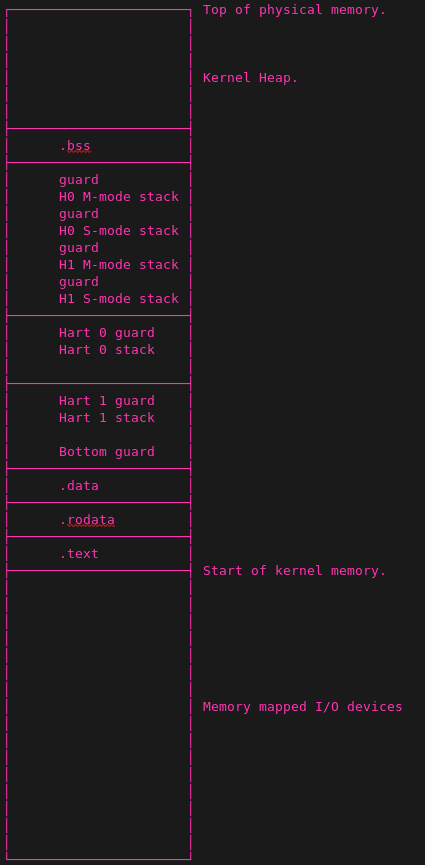
\includegraphics[height=0.9\textheight]{memlayout.png}
    \end{column}
  \end{columns}
\end{frame}

\begin{frame}[fragile]
  \frametitle{Allocation}
  \begin{columns}
    \begin{column}{0.5\textwidth}
      Memory allocation has two forms:
      \begin{itemize}
      \item \verb_palloc_ gives physically contiguous pages.\\
      \item \verb_vmalloc_ gives sub-page chunks like \verb_malloc_.\\
      \item Global alloc... Sound familiar?
      \end{itemize}
    \end{column}
    \begin{column}{0.5\textwidth}
        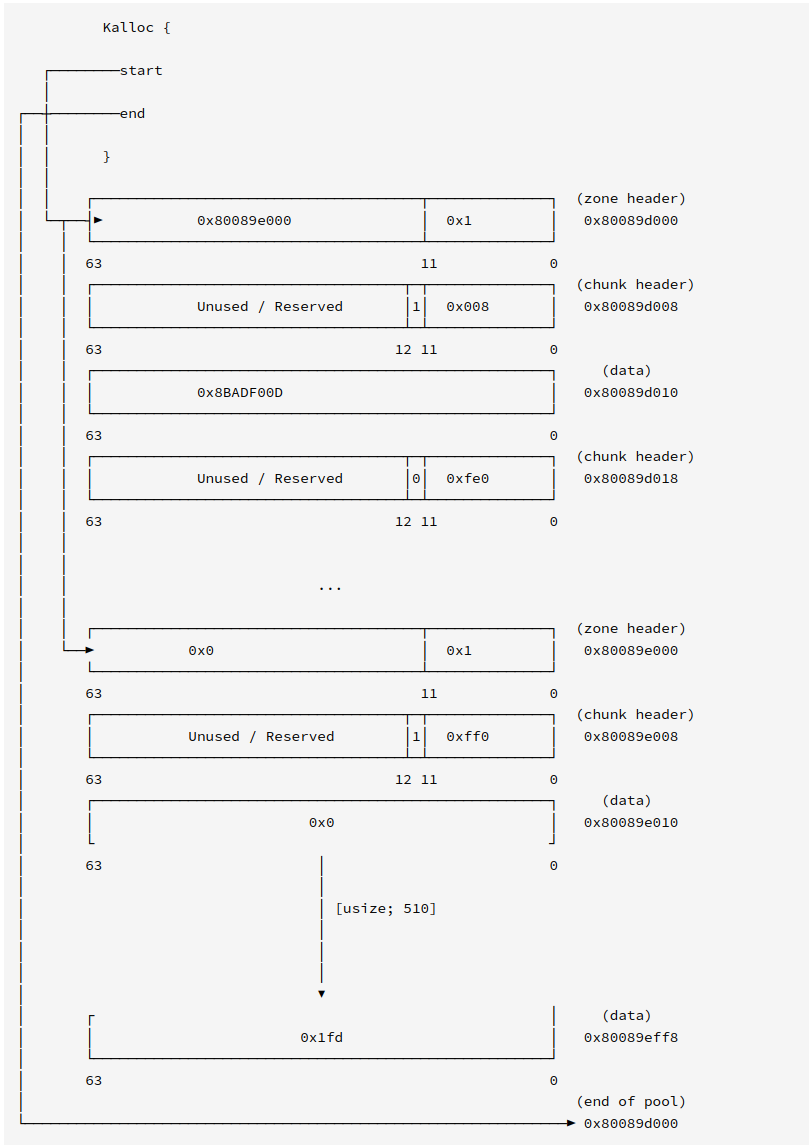
\includegraphics[height=0.8\textheight]{vmalloc_ascii.png}
    \end{column}
  \end{columns}
\end{frame}

\begin{frame}[fragile]
  \frametitle{Allocation Example}
  \begin{columns}
    \begin{column}{0.5\textwidth}
      Allocation on the kernel heap.
      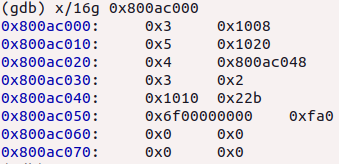
\includegraphics[width=\textwidth]{alloc_vmalloc.png}
    \end{column}
    \begin{column}{0.5\textwidth}
      Free from the kernel heap.
      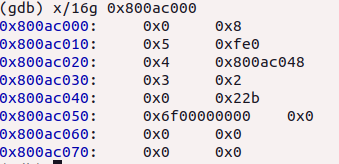
\includegraphics[width=\textwidth]{free_vmalloc.png}
    \end{column}
  \end{columns}
\end{frame}

\section{What You Can or Might Want To Use}

\begin{frame}[fragile]
  \frametitle{Useful tools}
  \begin{columns}
    \begin{column}{0.5\textwidth}
      Within reedos:
      \begin{itemize}
      \item The benefits of General Allocation: $\rightarrow$\\
      \item \verb`log` for logging with severity via uart.\\
      \item \verb`core::assert` for unsafe/runtime checking.
      \end{itemize}
    \end{column}
    \begin{column}{0.5\textwidth}
      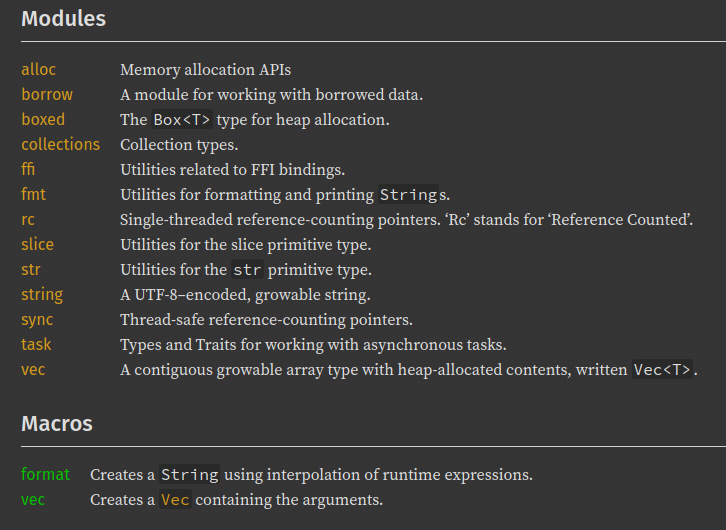
\includegraphics[width=\textwidth]{rustalloc.png}
    \end{column}
  \end{columns}
\end{frame}

\begin{frame}[fragile]
  \frametitle{Useful tools}
  Outside of reedos:
  \begin{itemize}
  \item GNU toolchain guides.\\
  \item Specifically GDB.\\
  \item Trust me use GDB.
  \end{itemize}
  \vspace{\baselineskip}
  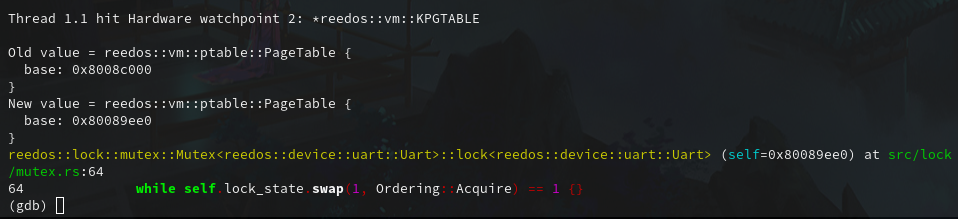
\includegraphics[width=\textwidth]{gdberror.png}
\end{frame}

\section{What You Could Do}
\begin{frame}
  \frametitle{What you could do / next steps}
  \begin{columns}
    \begin{column}{0.5\textwidth}
      Isolated / Reasonable projects:
      \begin{itemize}
      \item UART input and nice wrappers.\\
      \item File system (+ shell?).\\
      \item Device drivers.\\
      \item Page Fault handling (+ swap?).\\
      \item I/O device buffers.\\
      \item Syscalls.
      \end{itemize}
    \end{column}
    \begin{column}{0.5\textwidth}
      Connected / Difficult projects:
      \begin{itemize}
      \item UEFI + SiFive QEMU / Real Hardware.\\
      \item Network driver + stack.\\
      \item Rust async / threads (See scheduling).
      \end{itemize}
    \end{column}
  \end{columns}
\end{frame}


\end{document}
